% Figure from MATH 591 notes, section 8. Compile with the notes preamble.
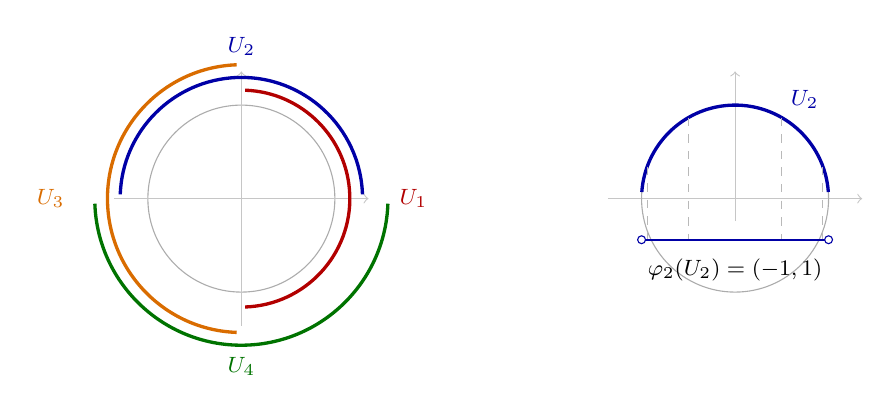
\begin{tikzpicture}[scale=0.95]
\draw[gray!65] (0,0) circle (1.25);
\draw[gray!45,->] (-1.7,0) -- (1.7,0); \draw[gray!45,->] (0,-1.7) -- (0,1.7);
\draw[red!70!black,very thick] (-88:1.45) arc (-88:88:1.45);
\draw[blue!65!black,very thick] (2:1.62) arc (2:178:1.62);
\draw[orange!85!black,very thick] (92:1.79) arc (92:268:1.79);
\draw[green!45!black,very thick] (182:1.96) arc (182:358:1.96);
\node[red!70!black,font=\footnotesize] at (2.3,0) {$U_1$};
\node[blue!65!black,font=\footnotesize] at (0,2.04) {$U_2$};
\node[orange!85!black,font=\footnotesize] at (-2.55,0) {$U_3$};
\node[green!45!black,font=\footnotesize] at (0,-2.24) {$U_4$};
\begin{scope}[xshift=6.6cm]
\draw[gray!45,->] (-1.7,0) -- (1.7,0); \draw[gray!45,->] (0,-0.3) -- (0,1.7);
\draw[gray!65] (0,0) circle (1.25);
\draw[blue!65!black,very thick] (4:1.25) arc (4:176:1.25);
\foreach \a in {20,60,120,160} { \draw[dashed,gray!55] (\a:1.25) -- ({1.25*cos(\a)},-0.55); }
\draw[blue!65!black,thick] (-1.25,-0.55) -- (1.25,-0.55);
\foreach \x in {-1.25,1.25} { \draw[blue!65!black,fill=white] (\x,-0.55) circle (1.5pt); }
\node[font=\footnotesize,anchor=north] at (0,-0.68) {$\varphi_2(U_2)=(-1,1)$};
\node[blue!65!black,font=\footnotesize] at (55:1.62) {$U_2$};
\end{scope}
\end{tikzpicture}
